\documentclass[a4paper]{scrartcl}
\usepackage[utf8]{inputenc}
\usepackage[ngermanb]{babel}
\usepackage{graphicx}
\usepackage{caption}
\usepackage{listings}
\usepackage{textcomp}

\usepackage[bookmarks=true, bookmarksopen=true, bookmarksnumbered=true, colorlinks=true, linkcolor=black, anchorcolor=black, citecolor=black, filecolor=black, menucolor=black, urlcolor=black]{hyperref}

\renewcommand{\familydefault}{\sfdefault}
\newcommand{\anf}[1]{\glqq{}#1\grqq{}}
\title{Handbuch zum XML-Backend}
\author{Christian Baumann}
\date{\today}

\begin{document}
  \maketitle
  
  \newpage
  
  \tableofcontents
  
  \newpage
  
	\section{Voraussetzungen}
	Um das XML-Backend nutzen zu können, müssen folgende Voraussetzungen erfüllt sein:
	\begin{itemize}
	  \item Plone
	  \item ECAutoAssessmentBox
	  \item ECSpooler
	  \item XML-Backend
	\end{itemize}
	Nachdem alle Komponenten, wie in den beiliegenden Anleitungen, installiert wurden, können Sie das Backend verwenden, indem Sie unter \texttt{Konfiguration} $\rightarrow$ \texttt{Auto Assessment Settings} den verfügbaren (\texttt{Available}) Backends \anf{\texttt{XML (\textit{Version})}} den gewählten (\texttt{Selected}) hinzufügen (vgl. Abbildung \ref{fig:addingXMLBackend}).
	
  \begin{center}
    \captionsetup{type=figure}
	  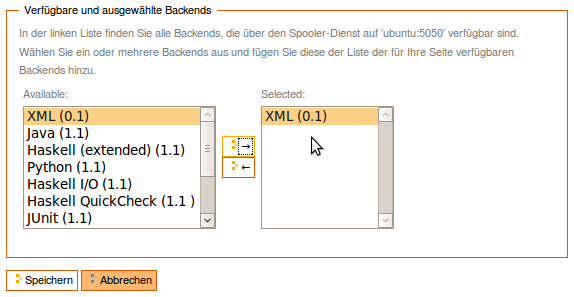
\includegraphics[width=1\textwidth]{images/AddingXMLBackend.png}
	  \captionof{figure}{Hinzufügen des XML-Backends.}
	  \label{fig:addingXMLBackend}
  \end{center}
	
	\section{Erstellen einer Aufgabe}
	  Im folgenden wird beschrieben, wie eine Aufgabe, die automatisch mit dem XML-Backend getestet werden soll, hinterlegt wird.
	  
	  \subsection{Erstellen eines EC-Ordners}
	    \begin{center}
        \captionsetup{type=figure}
	      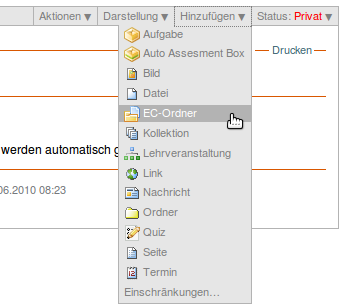
\includegraphics[width=0.5\textwidth]{images/AddingECFolder.png}
	      \captionof{figure}{Anlegen eines EC-Ordners.}
	      \label{fig:addingECFolder}
      \end{center}
      Aufgaben werden in Ordnern organisiert (vergleichbar mit einem Aufgabenblatt), die man wie folgt anlegt:
      
      Auf der Plone-Startseite befindet sich das Menü \anf{\texttt{Hinzufügen}}, in dem man den Punkt \anf{\texttt{EC-Ordner}} wählt.
      
      Es wird ein Titel, gefolgt von einer kurzen Beschreibung und optionalen Hinweisen angegeben. Durch einen Klick auf \anf{\texttt{Speichern}} werden die Eingaben bestätigt und ein neuer Ordner angelegt, in den automatisch gewechselt wird.
      \begin{center}
        \captionsetup{type=figure}
	      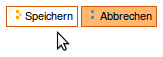
\includegraphics[scale=0.5]{images/Save.png}
	      \captionof{figure}{Speichern.}
	      \label{fig:save}
      \end{center}
	  
	  \subsection{Erstellen einer Aufgabe}
	  \begin{center}
        \captionsetup{type=figure}
	    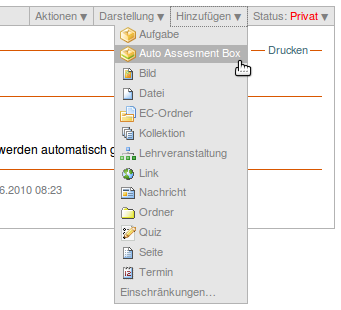
\includegraphics[width=0.50\textwidth]{images/AddingECAAB.png}
	    \captionof{figure}{Hinzufügen einer Auto Assesment Box.}
	    \label{fig:ecaab}
    \end{center}
	  Zur Erstellung einer Aufgabe wählen Sie aus dem Menü \anf{\texttt{Hinzufügen}} den Punkt \anf{\texttt{Auto Assesment Box}} und füllen auf der erscheinenden Seite die Eingabefelder wie gefordert aus.
	  Um das XML-Backend für diese Aufgabe nutzen zu können, wählen Sie unter dem Punkt \anf{\texttt{Backend}} \anf{\texttt{XML (\textit{Version})}} und bestätigen die Eingaben mit einem Klick auf \anf{\texttt{Speichern}}.
	  \subsection{Das XML-Backend}
	  Klicken Sie nun auf \anf{\texttt{Bearbeiten}}, gefolgt von \anf{\texttt{Backend}}.
	  
	  Das XML-Backend kann dazu genutzt werden, um Einreichungen von Studenten auf folgende Weisen zu testen:
	  \begin{itemize}
	    \item Wohlgeformtheit der Einreichung
	    \item Validität der Einreichung anhand einer DTD
	    \item Gleichheit von Ergebnissen von XPath-Anfragen
	  \end{itemize}
	  Hierzu sind einige Informationen im Backend zu hinterlegen:
  	  \subsubsection{Wohlgeformtheit}
  	  Um die Einreichung auf Wohlgeformtheit zu testen, aktiviert man die Checkbox \anf{\texttt{Test form}} (siehe Abbildung \ref{fig:form}).
  	  \begin{center}
        \captionsetup{type=figure}
	      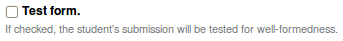
\includegraphics[width=0.50\textwidth]{images/Form.png}
	      \captionof{figure}{Checkbox zum aktivieren des Testens auf Wohlgeformtheit.}
	      \label{fig:form}
      \end{center}
      
  	  \subsubsection{DTD Validation}
  	  Um eine studentische Einreichung gegen eine DTD validieren zu lassen, benötigt das Backend eine hinterlegte DTD, die Sie im Feld \anf{\texttt{DTD}} (vgl. Abbildung \ref{fig:dtd}) angeben können.
  	  
  	  Studenten steht es frei, ihre lokale DTD nach eigenem Wunsch zu benennen. Das XML-Backend erkennt den lokalen DTD Namen und ersetzt ihn mit der serverseitig gespeicherten DTD.
  	  \begin{center}
        \captionsetup{type=figure}
	      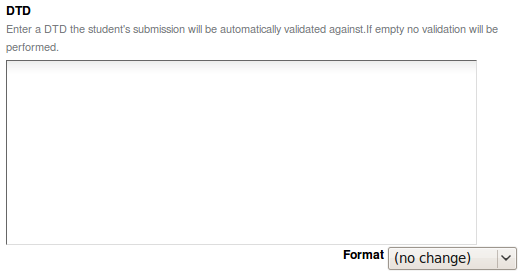
\includegraphics[width=0.75\textwidth]{images/DTD.png}
	      \captionof{figure}{Eingabefeld für eine DTD.}
	      \label{fig:dtd}
      \end{center}
  	  Beachten Sie, dass jede Eingabe in diesem Feld dazu führt, dass eine DTD Validation ausgeführt wird. Allein wenn dieses Feld leer ist, wird die DTD Validation übersprungen.
  	  
  	  \subsubsection{XPath-Anfragen}
  	  Das XML-Backend ist in der Lage XPath 2.0 Anfragen an eine studentische Einreichung zu stellen und diese mit einer Musterlösung zu vergleichen. Dazu hinterlegt man im Feld \anf{\texttt{Model solution}} (vgl. Abbildung \ref{fig:model}) die Modelllösung und im Feld \anf{\texttt{XPath statements}} (vgl. Abbildung \ref{fig:xpath}) zeilenweise XPath-Ausdrücke.
  	  
  	  \begin{center}
        \captionsetup{type=figure}
	      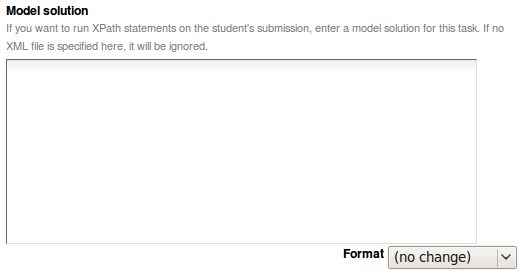
\includegraphics[width=0.75\textwidth]{images/Model.png}
	      \captionof{figure}{Eingabefeld für die Modelllösung.}
	      \label{fig:model}
      \end{center}
      
      Um als Lehrender die Dokumente in den XPath-Ausdrücken referenzieren zu können, wird die Variable \anf{\texttt{\$\{DOC\}}} verwendet, die intern in die tatsächlichen Dokumentennamen übersetzt wird.

      \begin{center}
        \captionsetup{type=figure}
	      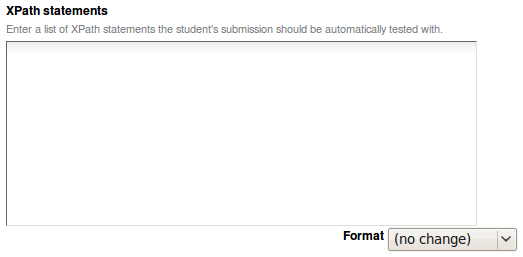
\includegraphics[width=0.75\textwidth]{images/XPath.png}
	      \captionof{figure}{Eingabefeld für XPath Ausdrücke.}
	      \label{fig:xpath}
      \end{center}
      Sind sowohl eine Modelllösung als auch XPath-Ausdrücke angegeben, wird automatisch ein XQuery-Programm generiert, das die Anfragen an die Musterlösung und die studentische Einreichung stellt und die Ergebnisse dieser vergleicht.
  	  
	\section{Beispiele}
	  Die folgenden Beispiele geben einen kurzen Einblick in die Funktionsweise des XML-Backends.
	  \subsection{Backend-Einstellungen}
	  Wir konfigurieren einen kompletten Test für dieses Beispiel, indem wir \anf{\texttt{Test form}} aktivieren, und folgende Texte in \anf{\texttt{DTD}}, \anf{\texttt{Model solution}} und \anf{\texttt{XPath statements}} hinterlegen.
	  
\begin{lstlisting}[language=XML, captionpos=b, frame=tlRB, caption={Beispiel DTD.}]
<!ELEMENT hallo (#PCDATA)>
\end{lstlisting}

\begin{lstlisting}[language=XML, captionpos=b, frame=tlRB, caption=Modelllösung.]
<?xml version="1.0" standalone="no"?>
<!DOCTYPE hallo SYSTEM "dtd.dtd">
<hallo>Hallo Welt!</hallo>
\end{lstlisting}

\begin{lstlisting}[language=XML, captionpos=b, frame=tlRB, caption={Beispiel XPath-Ausdrücke.}]
count(${DOC})
${DOC}/hallo
\end{lstlisting}
	  
	  \subsection{Einreichung}
  	  \subsubsection{Nicht wohlgeformt}
  	  Die Einreichung
  	  \begin{lstlisting}[language=XML, captionpos=b, frame=tlRB, caption={Nicht wohlgeformte Einreichung.}]
<?xml version="1.0" standalone="no"?>
<!DOCTYPE hallo SYSTEM "myLocal.dtd">
<hallo>Hallo Welt!</hallo
\end{lstlisting}
  	  führt zu der in Abbildung \ref{fig:notWellformed} dargestellten Rückmeldung.
  	  \begin{center}
        \captionsetup{type=figure}
	      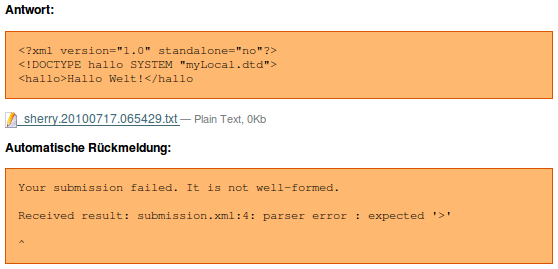
\includegraphics[width=0.75\textwidth]{images/notWellformed.png}
	      \captionof{figure}{Rückmeldung einer nicht wohlgeformten Einreichung.}
	      \label{fig:notWellformed}
      \end{center}
  	  
  	  \subsubsection{Nicht valide}
  	  Die Einreichung
  	  \begin{lstlisting}[language=XML, captionpos=b, frame=tlRB, caption={Nicht valide Einreichung.}]
<?xml version="1.0" standalone="no"?>
<!DOCTYPE hallo SYSTEM "myLocal.dtd">
<hola>Hallo Welt!</hola>
\end{lstlisting}
  	  führt zu der in Abbildung \ref{fig:notValid} dargestellten Rückmeldung.
  	  \begin{center}
        \captionsetup{type=figure}
	      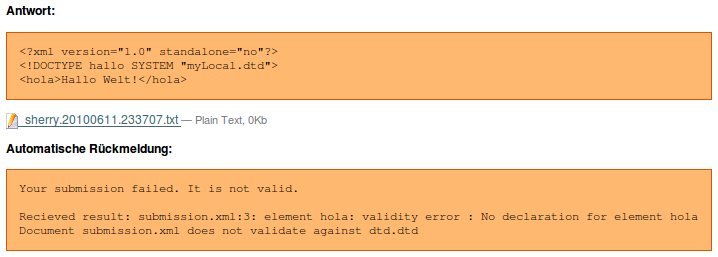
\includegraphics[width=0.8\textwidth]{images/notValid.png}
	      \captionof{figure}{Rückmeldung einer nicht validen Einreichung.}
	      \label{fig:notValid}
      \end{center}
      
      \subsubsection{Dokumentunterschiede}
      Die Einreichung
  	  \begin{lstlisting}[language=XML, captionpos=b, frame=tlRB, caption={Beispiel für eine semantisch falsche XML-Datei.}]
<?xml version="1.0" standalone="no"?>
<!DOCTYPE hallo SYSTEM "myLocal.dtd">
<hallo>Guten Tag Welt!</hallo>
\end{lstlisting}
      ist wohlgeformt und lässt sich gegen die hinterlegte DTD validieren. Allerdings sind die Textdaten innerhalb des \texttt{hallo}-Tags in der Einreichung von denen in der Modelllösung verschieden, was zu einer in Abbildung \ref{fig:notSameDocument} dargestellten Rückmeldung führt.
  	  \begin{center}
        \captionsetup{type=figure}
	      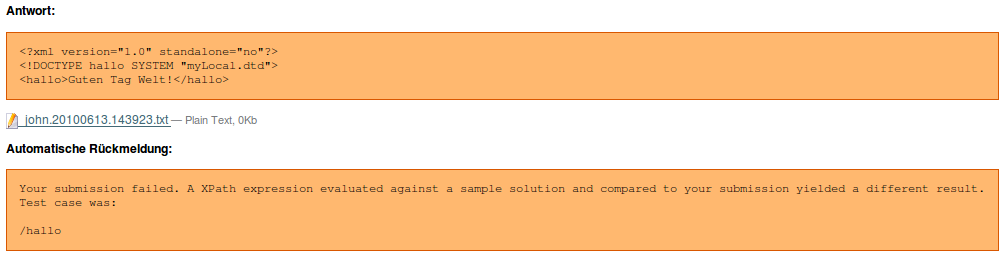
\includegraphics[width=1\textwidth]{images/notSameDocument.png}
	      \captionof{figure}{Rückmeldung bei Unterschieden in den verglichenen XML-Dateien nach einer XPath-Anfrage.}
	      \label{fig:notSameDocument}
      \end{center}
  	  
  	  \subsubsection{Fehlerfreie Einreichung}
  	  Die fehlerfreie Einreichung
  	  \begin{lstlisting}[language=XML, captionpos=b, frame=tlRB, caption={Fehlerfreie Einreichung}]
<?xml version="1.0" standalone="no"?>
<!DOCTYPE hallo SYSTEM "myLocal.dtd">
<hallo>Hallo Welt!</hallo>
\end{lstlisting}
  	  führt zu der in Abbildung \ref{fig:passed} dargestellten Rückmeldung.
  	  \begin{center}
        \captionsetup{type=figure}
	      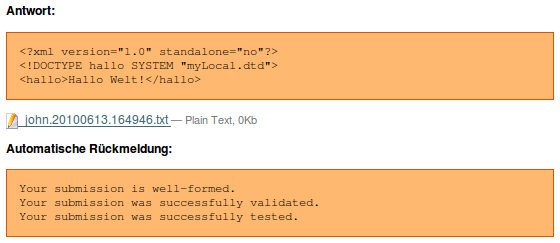
\includegraphics[width=0.8\textwidth]{images/passed.png}
	      \captionof{figure}{Rückmeldung im Falle einer fehlerfreien Einreichung.}
	      \label{fig:passed}
      \end{center}
\end{document}
